\documentclass[journal,compsoc]{IEEEtran}
% The preceding line is only needed to identify funding in the first footnote. If that is unneeded, please comment it out.
\usepackage[backend=biber]{biblatex}
\addbibresource{references.bib}
\usepackage{amsmath,amssymb,amsfonts}
\usepackage{algorithmic}
\usepackage{graphicx}
\usepackage{textcomp}
\usepackage{xcolor}
\usepackage{hyperref}
\usepackage{float}
\def\BibTeX{{\rm B\kern-.05em{\sc i\kern-.025em b}\kern-.08em
    T\kern-.1667em\lower.7ex\hbox{E}\kern-.125emX}}
\begin{document}

\title{Remembering and learning basic concepts \\
}

\maketitle

\section{Frequency}

Frequency is the number of occurrences of a repeating event per unit of time.

\[ f = \frac{1}{T} \] 

\section{Angular frequency}
In physics, angular frequency is a scalar measure of rotation rate. It refers to the angular displacement per unit time (for example, in rotation) or the rate of change of the phase of a sinusoidal waveform.
\[\omega = \frac{2\pi}{T} = 2\pi f \]

\section{Phase}
The phase of a periodic function \(F\) of some real variable \(t\) (such as time) is an angle-like quantity representing the fraction of the cycle covered up to \(t\). It is denoted \(\phi(t)\) and expressed in such a scale that it varies by one full turn as the variable \(t\) goes through each period.

The term "phase" is also used when comparing a periodic function \(F\) with a shifted version \(G\) of it. If the shift in \(t\) is expressed as a fraction of the period, and then scaled to an angle \(\varphi\) spanning a whole turn, one gets the phase shift, phase offset, or phase difference of \(G\) relative to \(F\).

\[\phi (t)=2\pi \left[\!\!\left[{\frac {t-t_{0}}{T}}\right]\!\!\right]\]

\section{Amplitude}
The amplitude of a periodic variable is a measure of its change in a single period (such as time or spatial period). There are various definitions of amplitude, which are all functions of the magnitude of the differences between the variable's extreme values. (see Fig. 1)

\begin{figure}[H]
\begin{center}
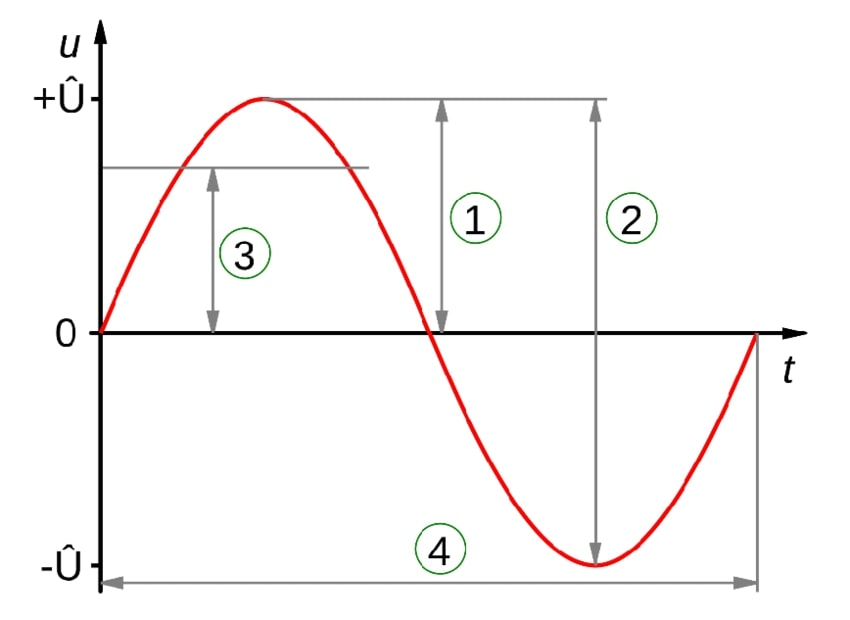
\includegraphics[scale=0.2]{amplitude}
		\caption{Peak amplitude (1), Peak-to-peak amplitude (2), Root-mean square amplitude (3), Wave period (4)}
\end{center}
\end{figure}

\section{Convolutions of signals}

A convolution is a mathematical operation applied on two functions which yields another function expressing how the shape of one is modified by the other. It is defined as the integral of the product of the two functions after one is reversed and shifted.

\[ (f * g)(t) = \int_{-\infty}^{\infty} f(\tau)g(t-\tau) \,d\tau \]

\section{Power}
In physics, power is the amount of energy transferred or converted per unit time (Joules per second).

\[ P = \frac{dW}{dt} \]

\section{Power spectrum}
The power spectrum \( S_{xx}(f)\) of a time series \(x(t)\) describes the distribution of power into frequency components composing that signal. According to Fourier analysis, any physical signal can be decomposed into a number of discrete frequencies, or a spectrum of frequencies over a continuous range. The statistical average of a certain signal or sort of signal (including noise) as analyzed in terms of its frequency content, is called its spectrum.

\section{Spectrogram}
A spectrogram is a visual representation of the spectrum of frequencies of a signal as it varies with time. A spectrogram can be generated by an optical spectrometer, a bank of band-pass filters, by Fourier transform or by a wavelet transform (in which case it is also known as a scaleogram or scalogram).

\begin{figure}[H]
\begin{center}
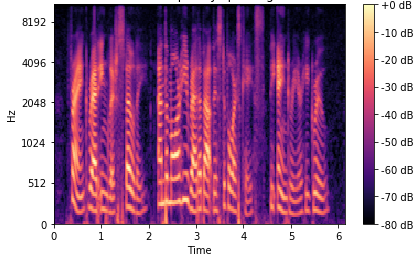
\includegraphics[scale=0.5]{spectrogram}
		\caption{Frequencies are shown increasing up the vertical axis, and time on the horizontal axis. The legend to the right shows that the color intensity increases with the sound intensity.}
\end{center}
\end{figure}

\section{Logarithmic scale}
A logarithmic scale (or log scale) is a way of displaying numerical data over a very wide range of values in a compact way - typically the largest numbers in the data are hundreds or even thousands of times larger than the smallest numbers. Such a scale is nonlinear: the numbers 10 and 20, and 60 and 70, are not the same distance apart on a log scale. Rather, the numbers 10 and 100, and 60 and 600 are equally spaced. Thus moving a unit of distance along the scale means the number has been multiplied by 10 (or some other fixed factor). Often exponential growth curves are displayed on a log scale, otherwise they would increase too quickly to fit within a small linear graph.

\section{Decibels}
The decibel is used in a wide range of applications. Decibels are especially used, when referring to power or a derived measure, whose values can vary in a wide range. The most prominent usage of decibels is in sound volume. So, for example a sound of 0dB is barely hearable, whereas a vacuum cleaner on average has 75dB and a rock concert reaches about 110dB.

When expressing a power ratio, it is defined as ten times the logarithm in base 10. That is, a change in power by a factor of 10 corresponds to a 10 dB change in level. When expressing root-power quantities, a change in amplitude by a factor of 10 corresponds to a 20 dB change in level.

Power:
\[ X_{dB} = 10\ log_{10}\left(\frac{X_{lin}}{X_{ref}}\right)\]

Amplitude:
\[ X_{dB} = 20\ log_{10}\left(\frac{X_{lin}}{X_{ref}}\right)\]

The equation transforms quantity \(X_{lin}\) from linear scale to a quantity in \(dB\) scale \(X_{dB}\). In order to do that, first the linear quantity is related to a reference quantity \(X_{ref}\) and the ratio of both is transformed into the log-domain. When \(X_{lin}\) equals the reference level, the dB-scale becomes zero.

\vspace{12pt}

\end{document}


